%!TEX encoding = IsoLatin
\chapter{Diagrammes Logiciel}
Les prochains diagrammes ont pour but de pr�senter l'id�e de d�part de notre architecture logicielle.
En effet, bien que ceci constitue notre architecture vis�e, cette derni�re changera in�luctablement lors du d�veloppement, comme le veut la gestion de projet "Agile".
Autre pr�cision, ces diagrammes repr�sentent seulement les tranches les plus utiles afin d'avoir une bonne vision de l'ensemble du syst�me.

\begin{figure}
  \centering
  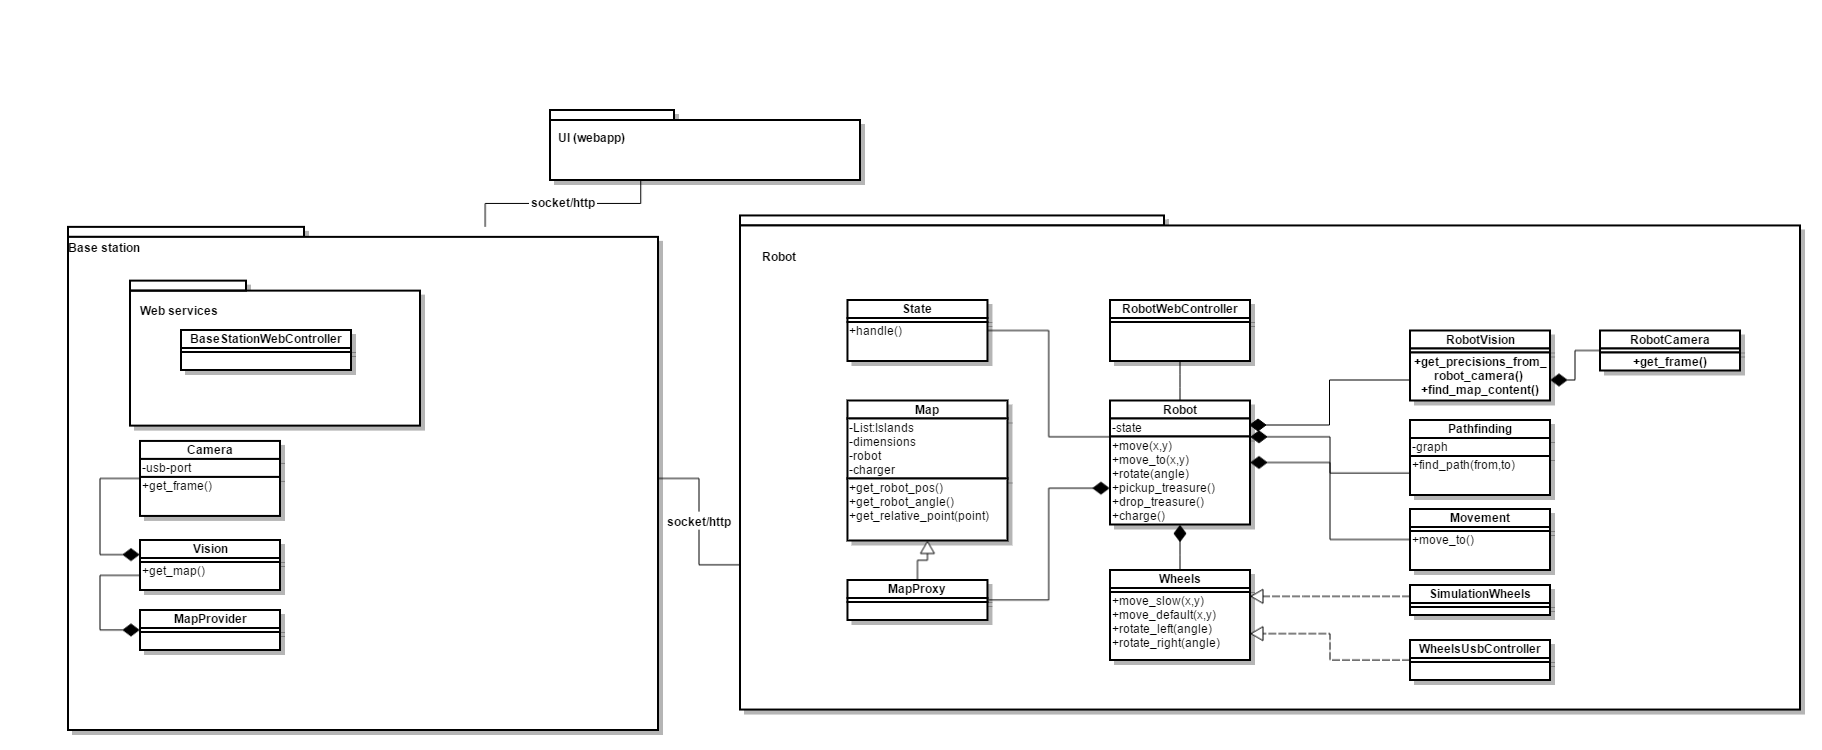
\includegraphics[scale=0.5, angle=90]{resources/diagrams/classDiagram.png}
  \caption{Diagramme de classe}
\end{figure}

\begin{figure}
  \centering
  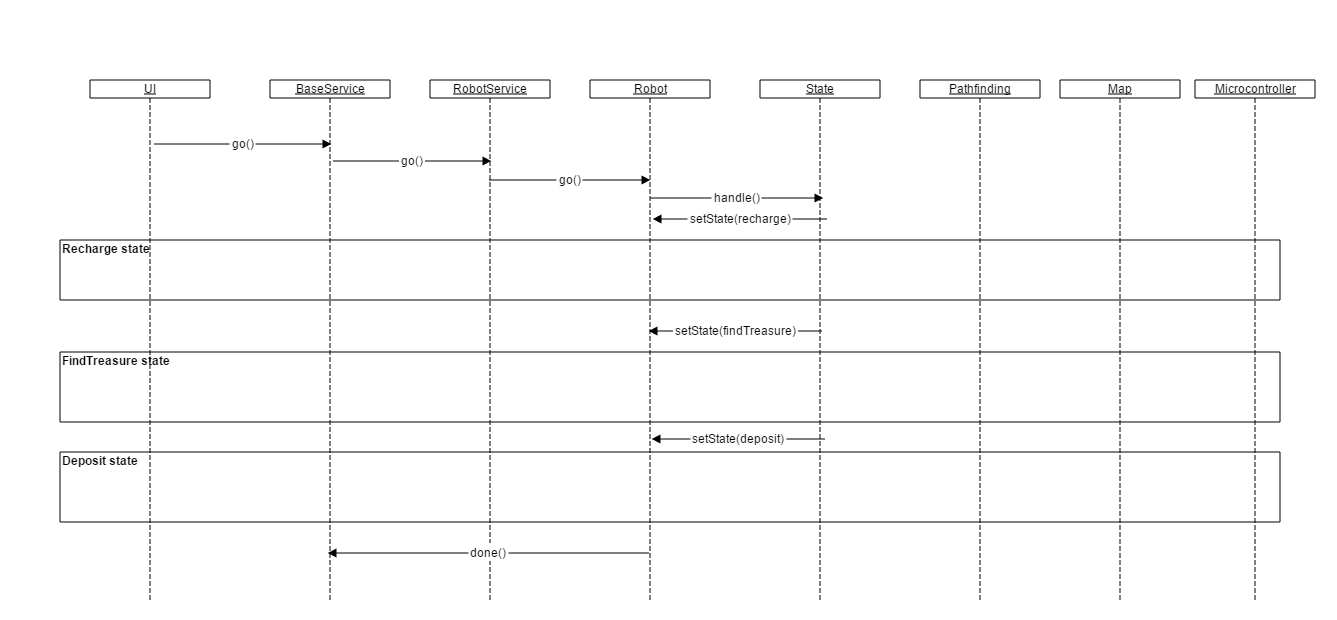
\includegraphics[scale=0.45, angle=90]{resources/diagrams/sequenceDiagram.png}
  \caption{Diagramme de S�quence complet}
\end{figure}

\begin{figure}
  \centering
  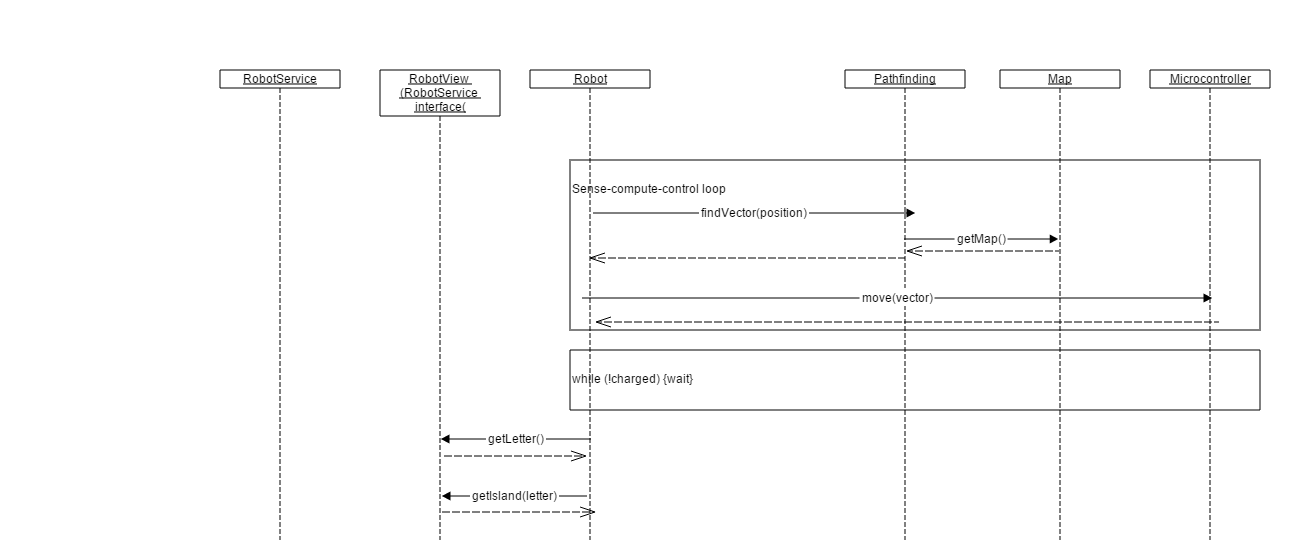
\includegraphics[scale=0.5, angle=90]{resources/diagrams/rechargeState.png}
  \caption{Diagramme de S�quence de recharge}
\end{figure}

\begin{figure}
  \centering
  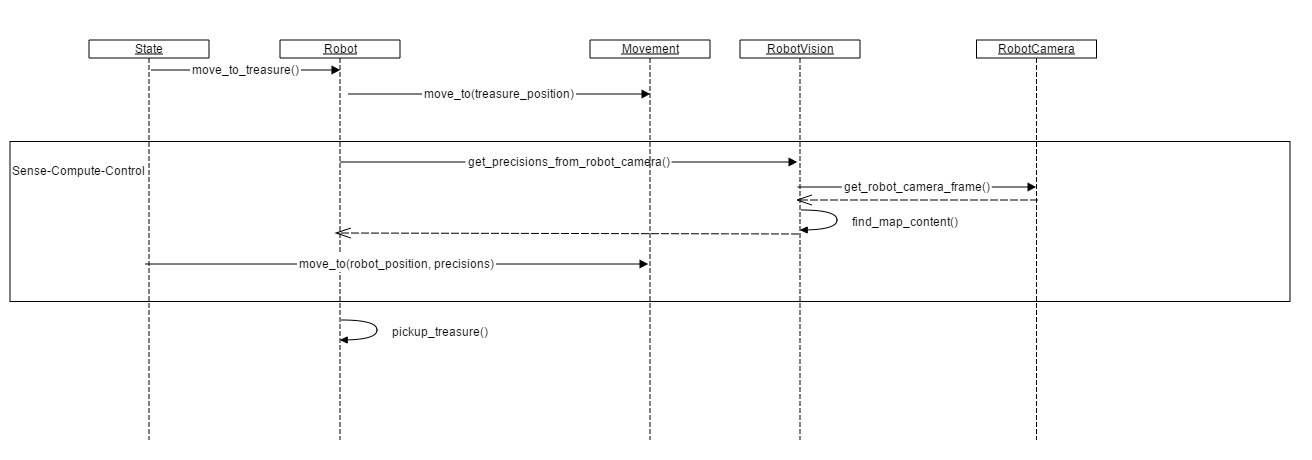
\includegraphics[scale=0.4, angle=90]{resources/diagrams/findTreasureState.png}
  \caption{Diagramme de S�quence de recherche de tr�sor}
\end{figure}

\begin{figure}
  \centering
  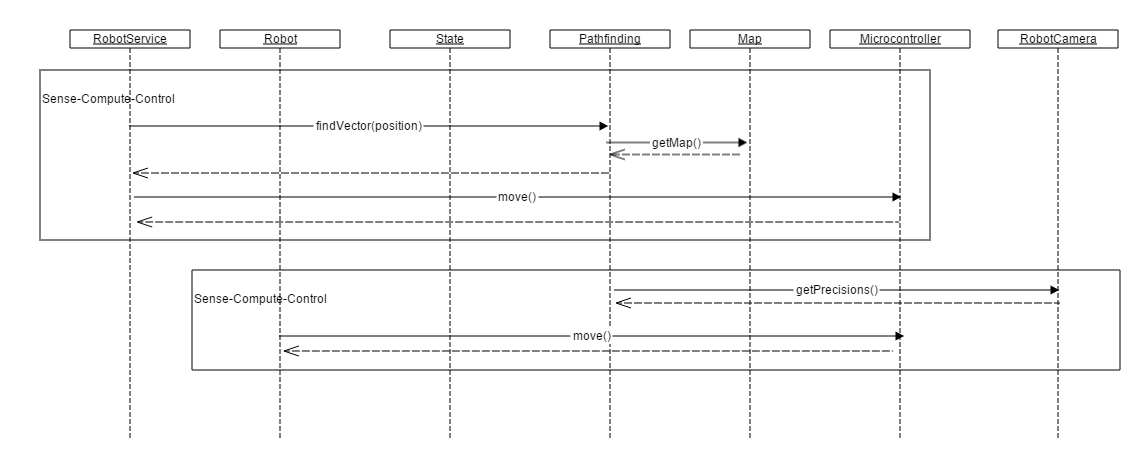
\includegraphics[scale=0.5, angle=90]{resources/diagrams/depositState.png}
  \caption{Diagramme de S�quence d�pot du tr�sor}
\end{figure}
